%%
%%  Hochschule für Technik und Wirtschaft Berlin --  Abschlussarbeit
%%
%%  Hauptdokument
%%
%%%%%%%%%%%%%%%%%%%%%%%%%%%%%%%%%%%%%%%%%%%%%%%%%%%

% Wichtige Pakete und Grundeinstellungen, verwendet Dokumentenklasse "scrbook" 
\documentclass[
		chapterprefix=false, 
		a4paper, 
		twoside, 
		parskip=half, 
		listof=totoc, 
		bibliography=totoc, 
		numbers=noendperiod, 
		captions=tableheading
]{scrbook}

%% Einstellungen und Anpassungen
%Anpassung der Seitenränder 
%% Geometrisches ...
\usepackage[inner=3cm]{geometry}
\makeatletter
\setlength\paperheight     {297mm}
\setlength\paperwidth  	   {210mm}
%\setlength\headheight      {2ex}
\setlength\headsep         {4ex} %2
\setlength\footskip        {35pt} %25
\setlength\textwidth       {155mm}
\setlength\textheight      {240mm} %245
%\setlength{\@tempdima}     {\paperwidth}
%\addtolength{\@tempdima}   {-2in}
%\addtolength{\@tempdima}   {-\textwidth}
%\setlength\oddsidemargin   {0.5\@tempdima} %replaced by 'inner'
%\setlength\evensidemargin  {\oddsidemargin} %replaced by 'inner'
%\setlength{\@tempdima}     {\paperheight}
%\addtolength{\@tempdima}   {-3in}
%\addtolength{\@tempdima}   {-\textheight}
%\setlength\topmargin       {.5\@tempdima}
\setlength\topmargin       {-1,2cm}
\setlength\footnotesep     {12\p@}
\setlength{\skip\footins}  {10\p@ \@plus 2\p@ \@minus 4\p@}
\setlength{\marginparsep}  {1pt}
\setlength{\marginparwidth}{20mm}
\makeatother 


%% Scalable fonts
\usepackage{lmodern}
%% set font size (needs to be loaded after \begin{document})
\AtBeginDocument{%
  \KOMAoption{fontsize}{11.5pt}%
%  \recalctypearea % not needed because use of geometry package
}
%% Unterstützung von Umlauten und anderen Sonderzeichen (UTF-8)
\usepackage{eurosym}
\usepackage[utf8]{inputenc}
\usepackage[T1]{fontenc}
\DeclareUnicodeCharacter{20AC}{\euro} %Euro-Symbol in UTF-8

%% Allgemeine Anpassungen 
\usepackage{scrhack} %Tweaks für scrbook
\usepackage[automark,headsepline]{scrlayer-scrpage} %Anpassung von Kopf- und Fußzeile
\usepackage{paralist}  %Kompakte Listen
%\usepackage[onehalfspacing]{setspace} %Zeilenabstand 1,5
\usepackage{setspace} %flexibler Zeilenabstand
\setstretch{1.15} %Zeilenabstand 1.15

\usepackage[stretch=10]{microtype} %Verbesserte Darstellung der Buchstaben zueinander
\usepackage{float} %Unterstützung fester Positionierung  (H)
\usepackage{csquotes} %wird von babel benötigt

%Glossar, Stichworverzeichnis (Akronyme als eigene Liste)
%\usepackage[toc, acronym]{glossaries} 

%% Mathematik:
\RequirePackage{amssymb, amsmath}
\RequirePackage{ifthen}
\RequirePackage{pifont} % Zapf Dingbats : https://ctan.ebinger.cc/tex-archive/macros/latex/required/psnfss/psnfss2e.pdf

%% Erweiterte Tabellen:
\usepackage{array, tabularx}
\setlength\extrarowheight{2pt} %extra Top-Padding in Latex-Tabellen
\usepackage{multirow}
\usepackage{longtable} %Umbrüche in Tabellen

%% Grafiken:
% Definition eigener Farben 
\usepackage[table,xcdraw]{xcolor}
\usepackage{tikz} % Vektorgrafiken, lädt graphicx automatisch
\usepackage{bmpsize} 

%Verknüpfungen im Dokument, Links werden durch "hidelink" nicht explizit hervorgehoben
%\PassOptionsToPackage{hyphens}{url}
\usepackage[hidelinks,german,hypertexnames=false]{hyperref}
%\hypersetup{breaklinks=true}
\usepackage{breakurl}
%\expandafter\def\expandafter\UrlBreaks\expandafter{\UrlBreaks% save the current one
%  \do\a\do\b\do\c\do\d\do\e\do\f\do\g\do\h\do\i\do\j%
%  \do\k\do\l\do\m\do\n\do\o\do\p\do\q\do\r\do\s\do\t%
%  \do\u\do\v\do\w\do\x\do\y\do\z\do\A\do\B\do\C\do\D%
%  \do\E\do\F\do\G\do\H\do\I\do\J\do\K\do\L\do\M\do\N%
%  \do\O\do\P\do\Q\do\R\do\S\do\T\do\U\do\V\do\W\do\X%
%  \do\Y\do\Z\do\*\do\-\do\~\do\'\do\"\do\-}%
  		% Import der Pakete und Stil des Dokuments
%%% Einstellungen zur Sprache und Silbentrennung im Dokument
%
% This is a document holding multiple languages.
% Switch between ENGLISH and GERMAN by commenting one of the following lines:
%\usepackage[ngerman,english]{babel} % makes ENGLISH content
\usepackage[english,ngerman]{babel} % makes GERMAN content
% this is the macro to define phrases in two languages:
\newcommand{\babel}[2]{\ifnum\pdfstrcmp{\languagename}{english}=0 {#2}\else{#1}\fi}
\newcommand{\DE}[1]{\ifnum\pdfstrcmp{\languagename}{ngerman}=0 {#1}\fi}
\newcommand{\EN}[1]{\ifnum\pdfstrcmp{\languagename}{english}=0 {#1}\fi}
% example:   \babel{Deutscher Text}{english text}
% example:   \DE{deutscher Text}
% example:   \EN{english text}
%%%%%%%%%%%%%%%


%%% Erstellung von Literaturverzeichnissen mit Biblatex (Biber/Bibtex)
% wählen Sie hier die für Ihr Latex-System nötige Literaturverarbeitung:
\usepackage[style=alphabetic, backend=biber,   natbib=true]{biblatex}  % Verarbeitung mit biber
%\usepackage[style=alphabetic, backend=bibtex, natbib=true]{biblatex}  % Verarbeitung mit bibtex
%
% Bibtex-Datei mit den Quellenangaben zur Arbeit
\addbibresource{references/references.bib}


%%% Abkürzungsverzeichnis
\usepackage[intoc]{nomencl}
\let\acro\nomenclature
\renewcommand{\nomname}{\babel{Abkürzungsverzeichnis}{Abbreviations}}
\setlength{\nomlabelwidth}{.25\hsize}
\renewcommand{\nomlabel}[1]{#1 \dotfill}
\setlength{\nomitemsep}{-\parsep}
\makenomenclature

%%% Überschriften auch in Times-Roman setzen
\addtokomafont{disposition}{\rmfamily}

%%% Kapitelnummer und Titel auf einer Zeile (erfordert die chapterprefix=false Option in class)
\renewcommand*{\chapterformat}{%
  \mbox{\chapapp~\thechapter:\enskip}%
}

%%% Farbdefinitionen
%  https://corporatedesign.htw-berlin.de/schrift-farbe/markenfarben/
\definecolor{HKS66}{RGB}{118,185,0}          %% HKS51, HTW-Grün
\definecolor{HKS47}{RGB}{0,130,209}      %% HKS47, HTW-Blau
\newcommand{\headcolor}{HKS66}
\newcommand{\alertcolor}{HKS47}
% Zusätzliche Farben
\definecolor{darkgreen}{RGB}{0,100,0}


%%% Stichwortverzeichnis 
\usepackage{imakeidx}
\makeatletter
\makeindex[columns=2, title=\babel{Stichwortverzeichnis}{Index}, options= -s settings/indexstyle.ist, intoc]
\makeatother
\indexsetup{level=\chapter*,toclevel=chapter}
% Pluszeichen in der Referenz beim Zitieren entfernen: [Kra+13] wird zu [Kra13]
\renewcommand*{\labelalphaothers}{}


%%% Darstellung von Quellcode incl. Syntax-Highlighting
\usepackage{listings}
\renewcommand{\lstlistlistingname}{\babel{Quelltextverzeichnis}{Listings}}
%Anpassungen zur Quellcodedarstellung
% muss bei Bedarf überschrieben werden (z.B. wenn unterschiedliche Sprachen zum Einsatz kommen)
\renewcommand{\lstlistingname}{Codeauszug}
\lstset{
	language=Python,
	numbers=left,
	columns=fullflexible,
	aboveskip=5pt,
	belowskip=10pt,
	basicstyle=\small\ttfamily,
	backgroundcolor=\color{black!5},
	commentstyle=\color{darkgreen},
	keywordstyle=\color{blue},
	stringstyle=\color{gray},
	showspaces=false,
	showstringspaces=false,
	showtabs=false,
	xleftmargin=16pt,
	xrightmargin=0pt,
	framesep=5pt,
	framerule=3pt,
	frame=leftline,
	rulecolor=\color{green},
	tabsize=2,
	breaklines=true,
	breakatwhitespace=true,
	prebreak={\mbox{$\hookleftarrow$}}
}

 	% Weitere Pakete und Anpassungen (Sprache, Quellenverwaltung, etc.)

% Variablendefinition und deren Voreinstellung festlegen
%

%% Variablen
\newboolean{@entwurfset}        \setboolean{@entwurfset}{true}
\newboolean{@abgabeset}         \setboolean{@abgabeset}{true}
\newboolean{@versionset}        \setboolean{@versionset}{true}
\newboolean{@versionsdatum}      \setboolean{@versionsdatum}{true}

%
\newcommand{\version}[1]{\setboolean{@versionset}{true} 
 \renewcommand{\theversion}{#1}} 
\newcommand{\datum}[1]{\renewcommand{\thedatum}{#1}}
\newcommand{\autor}[1]{\renewcommand{\theautor}{#1}}
\newcommand{\matrikelnr}[1]{\renewcommand{\thematrikelnr}{#1}}
\newcommand{\titel}[1]{\renewcommand{\thetitel}{#1}}
\newcommand{\untertitel}[1]{\renewcommand{\theuntertitel}{#1}}
\newcommand{\fachbereich}[1]{\renewcommand{\thefachbereich}{#1}}
\newcommand{\studiengang}[1]{\renewcommand{\thestudiengang}{#1}}
\newcommand{\thesistyp}[1]{\renewcommand{\thethesistyp}{#1}}
\newcommand{\abschluss}[1]{\renewcommand{\theabschluss}{#1}}
\newcommand{\firstExaminer}[1]{\renewcommand{\thefirstExaminer}{#1}}
\newcommand{\secondExaminer}[1]{\renewcommand{\thesecondExaminer}{#1}}
\newcommand{\betreuerFeld}[1]{\renewcommand{\thebetreuerFeld}{#1}}

%
\newcommand{\theversion}{0.0}      
\newcommand{\thedatum}{\today}
\newcommand{\theautor}{Autor angeben!}
\newcommand{\thematrikelnr}{123 456}
\newcommand{\thetitel}{Titel angeben!}
\newcommand{\theuntertitel}{}
\newcommand{\thefachbereich}{Fachbereich angeben}
\newcommand{\thestudiengang}{Studiengang angeben}
\newcommand{\thethesistyp}{Bachelorarbeit}
\newcommand{\theabschluss}{Bachelor of Engineering (B.Eng.)}
\newcommand{\thefirstExaminer}{Betreuer 1}
\newcommand{\thesecondExaminer}{Betreuer 2}
\newcommand{\thebetreuerFeld}{}

\betreuerFeld{
  \begin{tabular}{llr}
    Lecturer: & \thefirstExaminer \\
  \end{tabular}
}


%%%%%%%%%%%%%%%%%%%%%%%%%%%%%%%%
\renewcommand{\maketitle}{\htwTitelSeite}

%% Optionen

\DeclareOption{entwurf}
    {
      \setboolean{@entwurfset}{true}
      \setboolean{@abgabeset}{false}
    }

\DeclareOption{abgabe}
    {
      \setboolean{@entwurfset}{false}
      \setboolean{@abgabeset}{true}
    }



%% Setzen des defaults und verarbeiten
\ExecuteOptions{abgabe}     %TODO für Abgabe auf abgabe setzen
\ProcessOptions 

%%%%%%%%%%%%%%%%%%%%%%%%%%%%%%%%
%\newcommand{\hslogo}{pictures/Logo_HTW_Berlin.pdf}
%\newcommand{\hslogoscaled}[1]{{\mbox{\includegraphics[width=#1]\hslogo}}}

\newcommand{\hsfont}{}%    {\fontfamily{phv}\fontseries{m}\fontshape{n}\selectfont}
\newcommand{\hsheadfont}{}%{\fontfamily{phv}\fontseries{b}\fontshape{n}\selectfont}

\newcommand{\htwTitelSeite}
    {
      \thispagestyle{empty}
      \parindent=0pt
      \begin{minipage}[b]{0.65\textwidth}
       
        \ifthenelse{\boolean{@entwurfset}}
            {
              \begin{hsfont}
                \begin{tiny}
                  \raggedright
                  % Versionsnummer, wenn gesetzt
                  \ifthenelse{\boolean{@versionset}}
                       {Version \theversion\\}
                       {}
                       % Datum der letzten Änderung, falls gewünscht
	               \ifthenelse{\boolean{@versionsdatum}}
                       {letzte Änderung: \today \\}
		       {}
                \end{tiny}
              \end{hsfont}
            }
            {              
              % leer
              ~\hfill~
            }
      \end{minipage}
      
      \begin{minipage}[b]{0.35\textwidth}
      \vskip -2em
      \hfill  %\hslogoscaled{\textwidth}
%      \Ifpdfoutput{
%                  \message{PDF Output}
                  \mbox{
\includegraphics[width=\textwidth]{pictures/Logo_HTW_Berlin}}
%                  }{
%                 \mbox{
\includegraphics[width=\textwidth]{pictures/Logo_HTW_Berlin.eps}}
%                  \message{Kein PDF Output}
%                  }
      \end{minipage}

      \textcolor{HKS66}{\rule{\linewidth}{.4mm}}
      \vspace*{\stretch{1}}
      \begin{center}
        \begin{hsheadfont}
          \textcolor{\headcolor}{\LARGE \textbf{\thetitel}}
        \end{hsheadfont}
      \end{center}
      \vspace*{\stretch{0.5}}
      %
      \begin{hsheadfont}
        \begin{center}
          \textbf{\Large{\thethesistyp}}
        \end{center}
      \end{hsheadfont}
      \vspace*{\stretch{0.5}}
      %
      \begin{center}
        \begin{hsfont}
          from\\[2ex]
          {\textbf{\large\theautor}}\\[2ex]
          Matriculation number: \thematrikelnr\\[2ex]
          Faculty \thefachbereich\\
          of the Hochschule für Technik und Wirtschaft Berlin\\[2ex]
          Term paper in the course "Aktuelle Themen der Informatik" \\
          in the degree programme\\
          \textbf{\thestudiengang}
        \end{hsfont}
      \end{center}
     
      \vspace*{\stretch{1}}
       \begin{center}
         Day of delivery: \thedatum 
       \end{center}
         
      \vspace*{\stretch{1}}
      
      \thebetreuerFeld
      
      %
      \vspace*{\stretch{2}}

      \textcolor{HKS66}{\rule{\linewidth}{0.4mm}}\\[1.5ex]
       \begin{hsheadfont}
         % leer
         ~\hfill~
       \end{hsheadfont}
    }
    
		% Layout der Titelseite

%%%%%%%%%%%%%%%%%%%%%%%%%%%%%%%%%%%%%%%%%%%%%
% Im folgenden Bereich müssen Sie Anpassungen für das Deckblatt der Arbeit vornehmen!
%%%%%%%%%%%%%%%%%%%%%%%%%%%%%%%%%%%%%%%%%%%%%
%
%% Titel und Author 
\titel{Bootstrapping}
\autor{Hagen Wey}
\matrikelnr{s0575947}
%% Version und Abgabedatum
\version{0.2$\alpha$} 	%ToDo: wird derzeit noch nicht genutzt
\datum{16.07.2024}   	% Abgabedatum der Arbeit
%% Typ der Arbeit
\thesistyp{Term Paper}
%% Betreuer
\firstExaminer{Prof.~Dr. Tatiana Ermakova}
%% Fachbereich
\fachbereich{4 -- Informatik, Kommunikation und Wirtschaft --}
\studiengang{Angewandte Informatik}
%%%%%%%%%%%%%%%%%%%%%%%%%%%%%%%%%%%%%%%%%%%%%
% Ende des Bereichs für Anpassungen
%%%%%%%%%%%%%%%%%%%%%%%%%%%%%%%%%%%%%%%%%%%%%
%% Metadaten zu PDF hinzufügen
\hypersetup{
pdftitle = {\thetitel},
pdfsubject = {\thethesistyp},
pdfauthor = {\theautor},
%pdfkeywords = {Stichwort1, Stichwort2 ...} ,
pdfcreator = {LaTeX with hyperref},
pdfproducer = {pdflatex}
}
%% Pfad zu den Bildern
\graphicspath{
  {pictures/},
}
%% Current Bug-Fixes
% 2024-02 
% Error-Message ! Argument of \MT@gobble@to@nil has an extra }.
% https://tex.stackexchange.com/questions/702778/argument-of-mtgobbletonil-has-an-extra
\microtypesetup{nopatch=item}

%% Custom includes go here!!!



%%%%%%%%%%%%%%%%%%%%%%%%%%%%%%%%%%%%%%%%%%%%%
%% Start des Dokuments
%%%%%%%%%%%%%%%%%%%%%%%%%%%%%%%%%%%%%%%%%%%%%
\begin{document}

%% Deckblatt erzeugen
\maketitle

%% Inhaltsverzeichnis erstellen
\cleardoubleoddpage
\pagenumbering{Roman}
\tableofcontents \clearpage
%%%%%%%%%%%%%%%%%%%%%%%%%%%%%%%%%%%%%%%%%%%%%
%%%%%%%%%%%%%%%%%%%%%%%%%%%%%%%%%%%%%%%%%%%%%
%% In diesem Bereich müssen Sie Anpassungen für den Inhalt der Arbeit vornehmen!
%% Kurzzusammenfassung
\input{abstract_en.tex}

%% Hauptteil
\cleardoubleoddpage
\pagenumbering{arabic}


% !TEX root = ../Thesis.tex
%%
%%  Hochschule für Technik und Wirtschaft Berlin --  Abschlussarbeit
%%
%% Kapitel 1
%%
%%

\chapter{Introduction} \label{Introduction}


\section{Background and motivation} \label{Background and motivation}
In statistical analysis, bootstrapping is a method used for the derivation of robust estimates of standard errors and confidence intervals. This is applied to estimates such as mean, median, proportion, odds ratio, correlation coefficient or regression coefficient. Developed by Bradley Efron towards the end of the 1970s in "Bootstrap methods: another look at the jackknife" (1979), inspired by the jackknife technique, the bootstrap remains one of the most significant approaches in contemporary statistics, particularly as an alternative to parametric estimates.
The flexibility of this method in addressing uncertainty in estimates, particularly in the context of smaller or non-normally distributed samples, has made it a valuable tool in a range of business domains, including biostatistics, financial analysis and machine learning. This particular area is of outstanding importance for our course.
In this context, the topic of bootstrapping exemplifies the relationship between theoretical concepts and their practical application. This will be demonstrated later in the course through an example and an implementation of it. 


\section{Objectives of the paper}
The objective of this paper is to provide the reader with an insight into the concept of
bootstrapping. To this end, we will first elucidate some pivotal terminology and funda-
mental mathematical principles, with a view to fostering a more nuanced comprehension.
Thereafter, we will examine the structural underpinnings of bootstrapping and identify the
key elements that warrant consideration prior to reinvigorating the process through the use
of a theoretical exemplar. Finally, we will explore a potential implementation and utilize
this to elucidate the individual steps in what we term "plots".



% !TEX root = ../Thesis.tex
%%
%%  Hochschule für Technik und Wirtschaft Berlin --  Abschlussarbeit
%%
%% Kapitel 2 - Grundlagen
%%
%%


\chapter{Mathematical/statistical foundations of bootstrapping} \label{Foundations}


\section{Definition of terms}

\subsection{Standard error}
The standard error represents a significant statistical indicator, measuring the dispersion of sample mean values in relation to the true population value. It indicates the degree of accuracy with which the sample mean approximates the true population mean. A smaller standard error value indicates a more accurate estimate of the population mean by the sample mean. Conversely, a larger standard error value indicates an inaccurate estimate. 
The formula for the standard error is as follows: 
\[
SE = \frac{s}{\sqrt{n}}
\]
where \( s \) is the standard deviation of the sample and \( n \) is the sample size.

In the context of bootstrapping, the standard error is employed for the purpose of calculating confidence intervals for estimates. The aforementioned intervals indicate a range within which the true population parameter is likely to be situated with a high degree of probability. 


\subsection{Confidence intervalls}
Confidence intervals represent a fundamental concept in the field of statistics and constitute a crucial element of the bootstrap methodology. A confidence interval, or CI for short, represents the range within which a parameter (e.g. the mean value) is likely to fall with a certain probability. It is common practice among analysts to utilise confidence intervals that encompass either 95% or 99% of the anticipated observation.

The calculation of a confidence interval for the mean is typically performed as follows:
\[
\bar{x} \pm z^* \cdot SE
\]
where \( \bar{x} \) is the sample mean, \( z^* \) is the critical value from the standard normal distribution for the desired confidence level (e.g. 1.96 for a 95\% confidence interval) and \( SE \) is the standard error.


\section{Bootstrapping methodology}
Having established the two most crucial elements of bootstrapping and the means of calculating them, we may now proceed to the subject matter itself: bootstrapping. 

\subsection{Theory}
The fundamental concept of bootstrapping is the utilisation of sample data to infer conclusions regarding an estimated value (e.g. the sample mean) for a population parameter \( \theta\) (e.g. the population mean). Consequently, bootstrapping represents a methodology of replicate sampling. In this process, random samples are drawn independently of each other from existing sample data with the same sample size \(n\), from which conclusions can then be drawn.
This process enables the generation of empirical distributions and the calculation of confidence intervals. 



\begin{figure}[h]
    \centering
    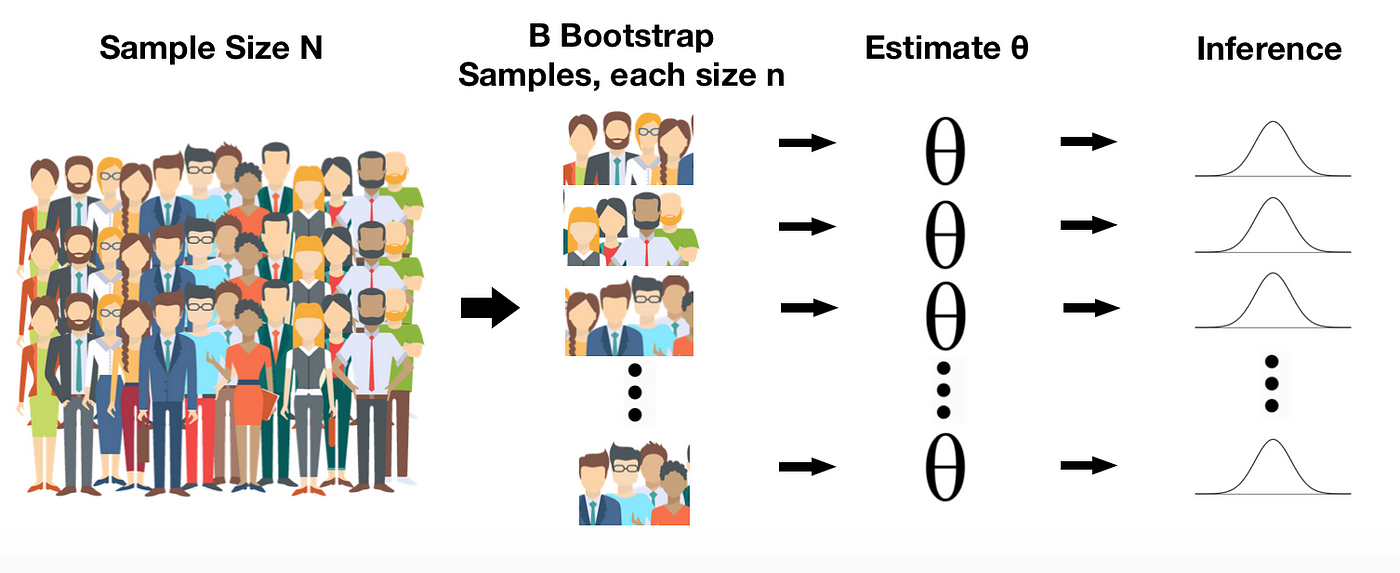
\includegraphics[width=\textwidth]{pictures/BootstrappingExample.png}
    \caption{Bootstrapping example}
    \label{fig:meinbild}
\end{figure}


Figure 2.1 provides a further illustration of the process in an abstract form. The accumulated knowledge, as illustrated in Figure 2.1, gives rise to the following process:

\begin{enumerate}
    \item \textbf{Drawing the bootstrap samples}:
    \begin{itemize}
        \item Assume we have a sample of \( n \) data points \( X = \{x_1, x_2, \ldots, x_n\} \).
        \item Draw \( B \) bootstrap samples from \( X \) with replacement. Each bootstrap sample has the same size as the original sample \( n \).
    \end{itemize}
    
    \item \textbf{Calculation of bootstraps}:
    \begin{itemize}
        \item For each of the \( B \) bootstrap samples, compute the desired statistic \( \hat{\theta}^* \) (e.g., mean, median, standard deviation).
    \end{itemize}
    
    \item \textbf{Estimation of the confidence interval}:
    \begin{itemize}
        \item Determine the \( (100 \cdot (1 - \alpha/2)) \)-th percentiles of the distribution of \( \hat{\theta}^* \) to obtain a \( (1 - \alpha) \)-confidence interval, where \( \alpha \) is the significance level.
    \end{itemize}
\end{enumerate}

\subsection{Example}
In order to provide a more illustrative example of the bootstrapping process, we will examine a fictitious case study from a practical context. 
In the field of medical research, bootstrapping represents a valuable methodology for estimating the standard error and calculating confidence intervals for a range of parameters. It is therefore appropriate to integrate this example into the medical problems sector, given that it is a topic that we always address in this course.

Let us consider a hypothetical scenario in which a research team is investigating the average efficacy of a novel pharmaceutical agent for the reduction of blood pressure in patients diagnosed with hypertension.

Steps of Bootstrapping:

\begin{enumerate}
    \item \textbf{Data collection}:
    \begin{itemize}
        \item A clinical trial was conducted by the research team, who collected a sample of 80 patients with hypertension who received the new drug.
    \end{itemize}
    
    \item \textbf{Application of the bootstrapping method}:
    \begin{itemize}
        \item \textbf{The bootstrap samples are drawn as follows:} A total of 1,000 bootstrap samples are drawn from the 80 available patient data sets.
        \item \textbf{Calculation of the bootstrap statistic:} The mean reduction in blood pressure following treatment is determined for each of the 1,000 bootstrap samples.
        \item \textbf{The estimation of the confidence interval is as follows: }The 95\% confidence interval for the mean blood pressure drop is determined by employing the 2.5\% and 97.5\% percentiles of the bootstrap mean values.
    \end{itemize}
    
    \item \textbf{Interpretation of the results}:
    \begin{itemize}
        \item The research team obtained a 95\% confidence interval for the average drop in blood pressure, for example, from 15 to 10 mmHg. This indicates that the actual mean reduction in blood pressure following treatment falls within this interval with 95\% confidence.
    \end{itemize}
\end{enumerate}

The utilisation of bootstrapping methodology allows the research team to make a well-founded assertion regarding the efficacy of the recently investigated pharmacological agent. This may subsequently result in the drug being approved or a similar outcome.
 
\section{Implementation results}
The conversion of this simple example into Python code allows the visualisation of the results. It should be noted that the values used in the code were randomly selected; this is merely an illustration of a fictitious example. 

\begin{figure}[h]
    \centering
    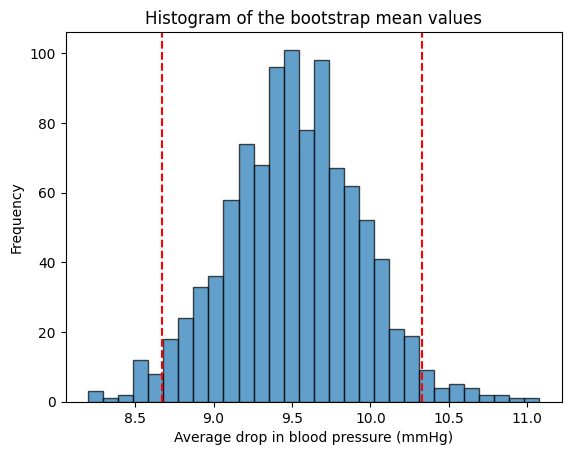
\includegraphics[width=\textwidth]{pictures/PlotBootstrappingExample.png}
    \caption{Bootstrapping example}
    \label{fig:meinbild}
\end{figure}

% !TEX root = ../Thesis.tex
%%
%%  Hochschule für Technik und Wirtschaft Berlin --  Abschlussarbeit
%%
%% Kapitel 5 - Tests
%%
%%

\chapter{Conclusion} \label{Conclusion}
A wide range of procedures and methods are employed in the field of statistics. While many of these techniques are more precise and comprehensive, it can be argued that bootstrapping is capable of achieving a level of statistical analysis that other methods are unable to match. It generates a substantial statistical analysis from a mere initial dataset. Furthermore, bootstrapping is relatively straightforward to comprehend and implement. The essential requirement is a computer with sufficient processing power to generate the requisite number of bootstraps and to perform the requisite mathematical operations. It is therefore my contention that bootstrapping represents one of the most powerful methods available for the analysis of small groups, particularly in the medical field, and the drawing of logical conclusions from them.

% !TEX root = ../Thesis.tex
%%
%%  Hochschule für Technik und Wirtschaft Berlin --  Abschlussarbeit
%%
%% Kapitel 6
%%
%%

\chapter{References} \label{References}

https://chrisbogner.github.io/datenanalyse/bootstrapping-und-konfidenzintervalle.html
https://de.wikipedia.org/wiki/Konfidenzintervall
https://datatab.de/tutorial/konfidenzintervall
https://www.investopedia.com/terms/c/confidenceinterval.asp
https://de.wikipedia.org/wiki/Standardfehler
https://dept.stat.lsa.umich.edu/~kshedden/introds/
https://www.ibm.com/docs/de/spss-statistics/saas?topic=bootstrapping-
https://towardsdatascience.com/an-introduction-to-the-bootstrap-method-58bcb51b4d60
https://jillian-green.medium.com/applications-of-bootstrapping-8240da9df6d7

\textbf{Link to Latex Template:}
https://github.com/tscheffl/HTW-Thesis

%% Diese Links sind leider in diesem Format nicht kompiliertbar:
%https://www.youtube.com/watch?v=JU5m-aPrNJw&t=64s



%% Anhang
%\cleardoubleoddpage
%\appendix
%% !TEX root = ../Thesis.tex
%%
%%  Hochschule für Technik und Wirtschaft Berlin --  Abschlussarbeit
%%
%% Anhang
%%
%%%%%%%%%%%%%%%%%%%%%%%%%%%%%%%%%%%%%%%%%%%%%%%%%%%%%%%%%%%%%%%%%%%%%


\chapter{Der Blindtext}


Weit hinten, hinter den Wortbergen, fern der Laender Vokalien und Konsonantien leben die Blindtexte. Abgeschieden wohnen Sie in Buchstabhausen an der Kueste des Semantik, eines grossen Sprachozeans. Ein kleines Baechlein namens Duden fliesst durch ihren Ort und versorgt sie mit den noetigen Regelialien. Es ist ein paradiesmatisches Land, in dem einem gebratene Satzteile in den Mund fliegen. Nicht einmal von der allmaechtigen Interpunktion werden die Blindtexte beherrscht - ein geradezu unorthographisches Leben.

Eines Tages aber beschloss eine kleine Zeile Blindtext, ihr Name war Lorem Ipsum, hinaus zu gehen in die weite Grammatik. Der grosse Oxmox riet ihr davon ab, da es dort wimmele von boesen Kommata, wilden Fragezeichen und hinterhaeltigen Semikoli, doch das Blindtextchen liess sich nicht beirren. Es packte seine sieben Versalien, schob sich sein Initial in den Guertel und machte sich auf den Weg. Als es die ersten Huegel des Kursivgebirges erklommen hatte, warf es einen letzten Blick zurueck auf die Skyline seiner Heimatstadt Buchstabhausen, die Headline von Alphabetdorf und die Subline seiner eigenen Strasse, der Zeilengasse. Wehmuetig lief ihm eine rethorische Frage ueber die Wange, dann setzte es seinen Weg fort.
Unterwegs traf es eine Copy. Die Copy warnte das Blindtextchen, da, wo sie herkaeme waere sie zigmal umgeschrieben worden und alles, was von ihrem Ursprung noch uebrig waere, sei das Wort und und das Blindtextchen solle umkehren und wieder in sein eigenes, sicheres Land zurueckkehren. Doch alles Gutzureden konnte es nicht ueberzeugen und so dauerte es nicht lange, bis ihm ein paar heimtueckische Werbetexter auflauerten, es mit Longe und Parole betrunken machten und es dann in ihre Agentur schleppten, wo sie es fuer ihre Projekte wieder und wieder missbrauchten. Und wenn es nicht umgeschrieben wurde, dann benutzen Sie es immernoch.
%%%%%%%%%%%%%%%%%%%%%%%%%%%%%%%%%%%%%%%%%%%%%
%%%%%%%%%%%%%%%%%%%%%%%%%%%%%%%%%%%%%%%%%%%%%
%%%%%%%%%%%%%%%%%%%%%%%%%%%%%%%%%%%%%%%%%%%%%

%% Abkürzungsverzeichnis
% 	Befehl: makeindex Thesis.nlo -s nomencl.ist -o Thesis.nls
%
%% Abbildungsverzeichnis
%\listoffigures \clearpage

%% Tabellenverzeichnis
%\listoftables \clearpage

%% Quelltextverzeichnis
%\lstlistoflistings \clearpage

%% Stichwortverzeichnis
%	Befehl: makeindex Thesis
%
%\printindex \clearpage

%% Literaturverzeichnis
%	Befehl: biber Thesis

%% Literaturverzeichnis
%\printbibliography[heading=bibintoc, title={Literaturverzeichnis}]
%\printbibliography[heading=bibintoc, keyword={online}, title={Onlinequellen}]\clearpage


%\printbibliography[heading=bibintoc, title={Literaturverzeichnis}]
%\clearpage
%Literaturverzeichnisse getrennt nach Stichwort
%\printbibliography[heading=bibintoc, keyword={book}, title={Literaturverzeichnis}]\clearpage
%\printbibliography[heading=bibintoc, keyword={online}, title={Onlinequellen}]\clearpage
%\printbibliography[heading=bibintoc, keyword={image}, title={Bildquellen}]\clearpage

\end{document}
